
\documentclass[11pt]{scrreprt}

\usepackage{graphicx} 
\usepackage{ucs}
\usepackage[utf8x]{inputenc}
\usepackage[T1]{fontenc}
\usepackage[ngerman]{babel}
\usepackage{amsmath}
 
 
\begin{document}
Im Rahmen der Aufgabe wurden verschiedene Implementierungen eines Matrix-Vektor-Produkts $A*x$ im Hinblick auf ihre Laufzeit miteinander verglichen. Folgende Implementierungsmöglichkeiten wurden betrachtet:

\begin{itemize}
\item Serielles Berechnen von $Ax$ auf der CPU
\item Serielles Berechnen von $A^T  x$ auf der CPU
\item Paralleles Berechnen von $Ax$ auf der GPU
\item Paralleles Berechnen von $A^T  x$ auf der GPU
\item Paralleles Berechnen von $Ax$ auf der GPU unter Nutzung von shared memory
\item Paralleles Berechnen von $A^T x$ auf der GPU unter Nutzung von shared memory
\item Paralleles Berechnen von $Ax$ auf der GPU unter Nutzung von shared memory und dynamic parallelism
\item Paralleles Berechnen von $A^T  x$ auf der GPU unter Nutzung von shared memory und dynamic parallelism
\end{itemize}
Abbildung \ref{im:times} zeigt die Laufzeiten der verschiedenen Implementierungen in Millisekunden für verschiedene Matrix-Größen. 

In den Abbildungen \ref{im:graph_full}, \ref{im:graph_smallx} und \ref{im:graph_smalltime} sind die verschiedenen Laufzeiten in Abhängigkeit von der Matrixgröße dargestellt.

\begin{figure}
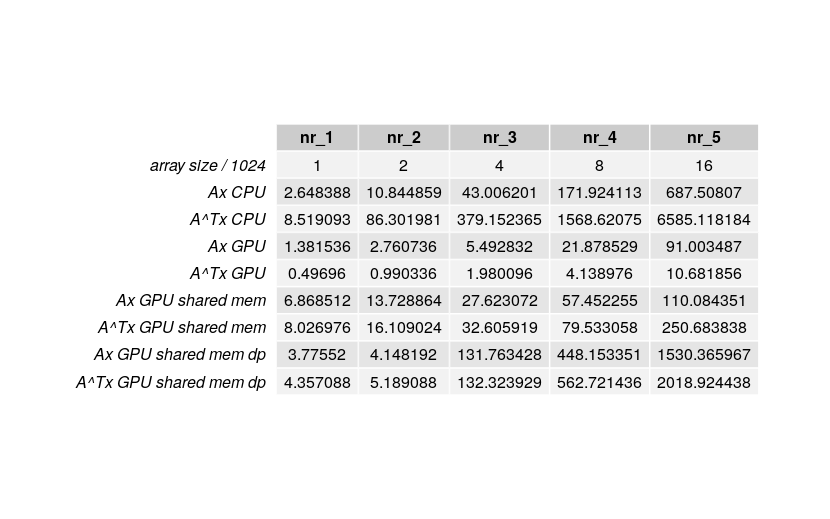
\includegraphics[width = \textwidth]{bilder/times.png}
\caption{Laufzeiten(ms) der verschiedenen Implementierungen für verschiedene Matrixgrößen}\label{im:times}
\end{figure}
\begin{figure}
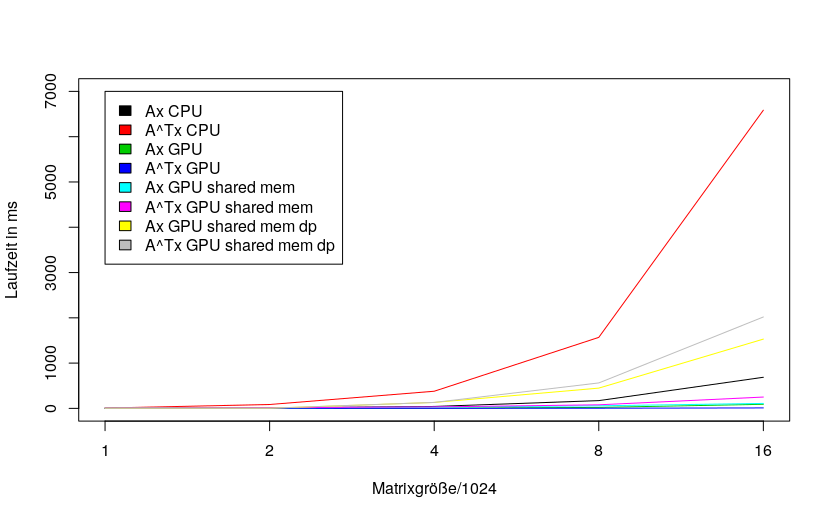
\includegraphics[width = \textwidth]{bilder/graph_full.png}
\caption{Entwicklung der Laufzeiten}
\label{im:graph_full}
\end{figure}
\begin{figure}
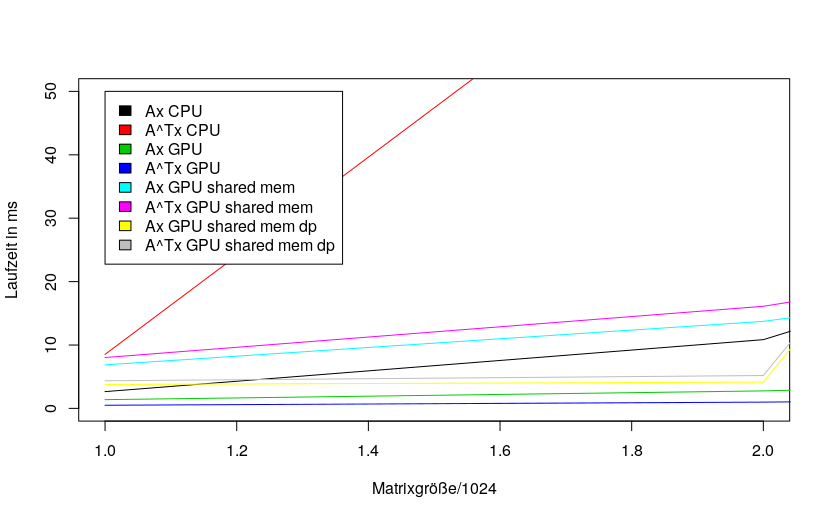
\includegraphics[width = \textwidth]{bilder/graph_smallx.png}
\caption{Entwicklung der Laufzeiten bei kleinen Problemgrößen}
\label{im:graph_smallx}
\end{figure}
\begin{figure}
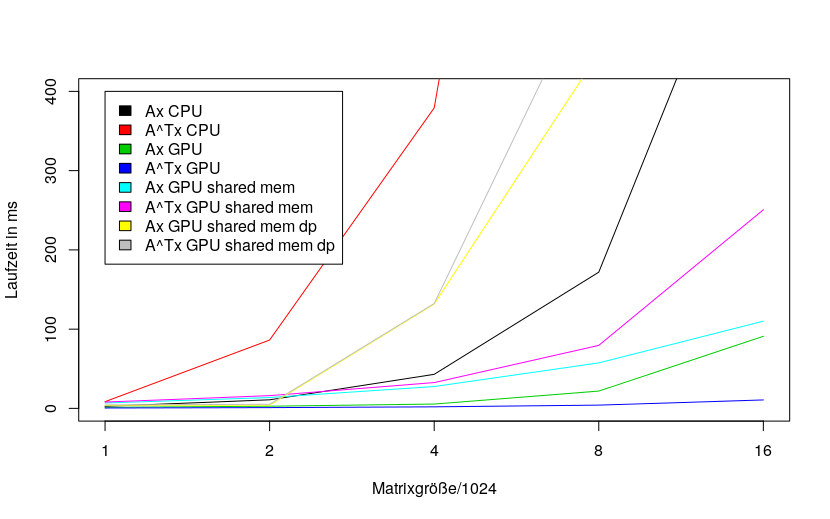
\includegraphics[width = \textwidth]{bilder/graph_smalltime.png}
\caption{Entwicklung der Laufzeiten unter 400 ms}
\label{im:graph_smalltime}
\end{figure}

\end{document}